\documentclass[12pt]{article}
\usepackage[utf8]{inputenc}
\usepackage[catalan]{babel}
\usepackage{amsmath, amssymb, amsfonts}
\usepackage{geometry}
\usepackage{fancyhdr}
\usepackage{tikz}
\usetikzlibrary{matrix, calc}
\usepackage{tcolorbox}
\usepackage[colorlinks=true, linkcolor=blue]{hyperref}

\setlength{\headheight}{15pt}

\geometry{a4paper, left=2cm, right=2cm, top=2.5cm, bottom=2.5cm}

\pagestyle{fancy}
\fancyhf{}
\fancyhead[L]{Matemàtiques 2n Batxillerat}
\fancyhead[R]{Matrius i determinants}
\fancyfoot[L]{\href{mailto:orodri11@xtec.cat}{orodri11@xtec.cat}}
\fancyfoot[R]{\thepage}

% Estils per a quadres
\newtcolorbox{concept}[1][]{colback=blue!5!white, colframe=blue!75!black, fonttitle=\bfseries, title=Concepte, #1}
\newtcolorbox{exemple}[1][]{colback=green!5!white, colframe=green!75!black, fonttitle=\bfseries, title=Exemple, #1}
\newtcolorbox{exercici}[1][]{colback=yellow!5!white, colframe=yellow!75!black, fonttitle=\bfseries, title=Exercici, #1}

% Per a les matrius en negreta
\newcommand{\mat}[1]{\mathbf{#1}}
\newcommand{\vect}[1]{\mathbf{#1}}

\begin{document}

% Portada
\begin{titlepage}
    \centering
    {\Huge \textbf{Matrius i determinants \\ 2n Batxillerat} \par}
    \vspace{1cm}
    % 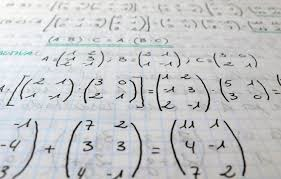
\includegraphics[width=0.5\textwidth]{matrius.png}
    \vspace{1cm}
    \tableofcontents
\end{titlepage}

\newpage

\section{Matrius. Primeres definicions}

\subsection{Definició d'una matriu}
\begin{concept}
Una matriu és una disposició rectangular d'elements (nombres, variables o expressions) ordenats en files i columnes. Cada element d'una matriu es denota per $a_{ij}$, on $i$ indica la fila i $j$ la columna.
\end{concept}

\subsection{Matriu numèrica}
\begin{concept}
Una matriu numèrica de dimensió $m \times n$ és un conjunt de nombres reals disposats en $m$ files i $n$ columnes:
\[
\mat{A} = 
\begin{pmatrix}
a_{11} & a_{12} & \cdots & a_{1n} \\
a_{21} & a_{22} & \cdots & a_{2n} \\
\vdots & \vdots & \ddots & \vdots \\
a_{m1} & a_{m2} & \cdots & a_{mn}
\end{pmatrix}
\]
Aquests nombres es diuen \textbf{components} o \textbf{elements} de la matriu. Les matrius es representen amb lletres majúscules, i els seus elements amb lletres minúscules. Cada element s'identifica amb dos subíndexs: el primer indica la \textbf{fila} i el segon la \textbf{columna}.
\end{concept}

\subsection*{Exemple de dimensió d'una matriu}
\begin{exemple}
La matriu 
\[
\mat{A} = \begin{pmatrix}
1 & 2 & 3 \\
4 & 5 & 6
\end{pmatrix}
\]
és de dimensió $2 \times 3$ perquè té 2 files i 3 columnes.
\end{exemple}

\subsection{Igualtat de matrius}
\begin{concept}
Dues matrius $\mat{A}$ i $\mat{B}$ són iguals si:
\begin{itemize}
    \item Tenen la mateixa dimensió $m \times n$.
    \item Els elements corresponents són iguals, és a dir, $a_{ij} = b_{ij}$ per a tot $i$ i $j$.
\end{itemize}
\end{concept}

\subsection*{Exercicis resolts i proposats}
\begin{exercici}
Escriu la matriu $\mat{A} = (a_{ij})$ de dimensió $4 \times 2$ on $a_{ij} = i - 3j$.

\textbf{Solució:}
\[
\mat{A} = \begin{pmatrix}
-2 & -5 \\
-1 & -4 \\
0 & -3 \\
1 & -2
\end{pmatrix}
\]

Escriu la matriu $\mat{B} = (b_{ij})$ de dimensió $4 \times 3$ on $b_{ij} = i \cdot j$.

\textbf{Solució:}
\[
\mat{B} = \begin{pmatrix}
1 & 2 & 3 \\
2 & 4 & 6 \\
3 & 6 & 9 \\
4 & 8 & 12
\end{pmatrix}
\]

Escriu la matriu $\mat{C} = (c_{ij})$ de dimensió $2 \times 4$ on $c_{ij} = (-1)^i + (-1)^j$.

\textbf{Solució:}
\[
\mat{C} = \begin{pmatrix}
-2 & 0 & 0 & -2 \\
0 & -2 & -2 & 0
\end{pmatrix}
\]

Escriu la matriu $\mat{D} = (d_{ij})$ de dimensió $3 \times 3$ on $d_{ij} = i^j$.

\textbf{Solució:}
\[
\mat{D} = \begin{pmatrix}
1 & 1 & 1 \\
2 & 4 & 8 \\
3 & 9 & 27
\end{pmatrix}
\]
\end{exercici}

\subsection{Matriu transposada}
\begin{concept}
La transposada d'una matriu $\mat{A}$, denotada per $\mat{A}^T$, s'obté intercanviant les files i les columnes de $\mat{A}$.

\textbf{Exemple:}
Si
\[
\mat{A} = \begin{pmatrix}
1 & 2 & 3 \\
4 & 5 & 6
\end{pmatrix}
\]
la seva transposada és
\[
\mat{A}^T = \begin{pmatrix}
1 & 4 \\
2 & 5 \\
3 & 6
\end{pmatrix}
\]
\end{concept}

\subsection{Propietats de les matrius oposades i transposades}
\begin{concept}
Relacionades amb les matrius oposades i transposades tenim les següents propietats:
\[
-(-\mat{A}) = \mat{A}
\]
\[
(\mat{A}^T)^T = \mat{A}
\]
\[
-(\mat{A}^T) = (-\mat{A})^T
\]

\textbf{Nota:} Hi ha diferents notacions per a la matriu transposada:
\begin{itemize}
    \item $\mat{A}^T$
    \item $\mat{A}^t$
    \item $^T\mat{A}$
\end{itemize}
\end{concept}

\section{Matrius quadrades}

\subsection{Matriu quadrada}
\begin{concept}
Una matriu quadrada és una matriu que té el mateix nombre de files i columnes, és a dir, de dimensió $n \times n$.
\end{concept}

\begin{exemple}
La següent matriu és una matriu quadrada de dimensió $3 \times 3$:
\[
\mat{A} = \begin{pmatrix}
1 & 2 & 3 \\
4 & 5 & 6 \\
7 & 8 & 9
\end{pmatrix}
\]
\end{exemple}

\subsection{Diagonals i traça d'una matriu quadrada}
\begin{concept}
- La \textbf{diagonal principal} d'una matriu quadrada són els elements $a_{ii}$, on $i = 1, 2, \dots, n$.  
- La \textbf{diagonal secundària} són els elements situats en $a_{i, n+1-i}$, per $i = 1, 2, \dots, n$.  
- La \textbf{traça} d'una matriu quadrada és la suma dels elements de la diagonal principal:
\[
\text{traça}(\mat{A}) = \sum_{i=1}^n a_{ii}
\]
\end{concept}

\begin{exemple}
Sigui la matriu quadrada:
\[
\mat{A} = \begin{pmatrix}
1 & 2 & 3 \\
4 & 5 & 6 \\
7 & 8 & 9
\end{pmatrix}
\]
- La diagonal principal és $1, 5, 9$.
- La diagonal secundària és $3, 5, 7$.
- La traça de $\mat{A}$ és:
\[
\text{traça}(\mat{A}) = 1 + 5 + 9 = 15
\]
\end{exemple}

\subsection{Matrius triangulars}
\begin{concept}
- Una matriu és \textbf{triangular superior} si tots els elements per sota de la diagonal principal són zero.
- Una matriu és \textbf{triangular inferior} si tots els elements per sobre de la diagonal principal són zero.
\end{concept}

\begin{exemple}
Exemple d'una matriu triangular superior:
\[
\mat{A} = \begin{pmatrix}
1 & 2 & 3 \\
0 & 4 & 5 \\
0 & 0 & 6
\end{pmatrix}
\]
Exemple d'una matriu triangular inferior:
\[
\mat{B} = \begin{pmatrix}
1 & 0 & 0 \\
2 & 3 & 0 \\
4 & 5 & 6
\end{pmatrix}
\]
\end{exemple}

\subsection{Matrius diagonals}
\begin{concept}
Una matriu diagonal és una matriu quadrada en què tots els elements fora de la diagonal principal són zero.
\end{concept}

\begin{exemple}
La següent matriu és una matriu diagonal:
\[
\mat{A} = \begin{pmatrix}
1 & 0 & 0 \\
0 & 5 & 0 \\
0 & 0 & 9
\end{pmatrix}
\]
\end{exemple}

\subsection{Matrius simètriques i antisimètriques}
\begin{concept}
- Una matriu quadrada $\mat{A}$ és \textbf{simètrica} si $\mat{A}^T = \mat{A}$
- Una matriu quadrada $\mat{A}$ és \textbf{antisimètrica} si $\mat{A}^T = -\mat{A}$
\end{concept}

\begin{exemple}
Exemple de matriu simètrica:
\[
\mat{A} = \begin{pmatrix}
1 & 2 & 3 \\
2 & 4 & 5 \\
3 & 5 & 6
\end{pmatrix}, \quad \mat{A}^T = \mat{A}
\]
Exemple de matriu antisimètrica:
\[
\mat{B} = \begin{pmatrix}
0 & -2 & -3 \\
2 & 0 & -4 \\
3 & 4 & 0
\end{pmatrix}, \quad \mat{B}^T = -\mat{B}
\]
\end{exemple}

\subsection*{Exercicis resolts}
\begin{exercici}
1. Calcula la traça de la matriu:
\[
\mat{A} = \begin{pmatrix}
3 & 2 & 1 \\
0 & 4 & 5 \\
7 & 8 & 6
\end{pmatrix}
\]

\textbf{Solució:}
La traça de $\mat{A}$ és:
\[
\text{traça}(\mat{A}) = 3 + 4 + 6 = 13.
\]

2. Verifica si la següent matriu és simètrica:
\[
\mat{B} = \begin{pmatrix}
1 & 2 & 3 \\
2 & 4 & 5 \\
3 & 5 & 6
\end{pmatrix}
\]

\textbf{Solució:}
Es calcula la transposada:
\[
\mat{B}^T = \begin{pmatrix}
1 & 2 & 3 \\
2 & 4 & 5 \\
3 & 5 & 6
\end{pmatrix}
\]
Com que $\mat{B}^T = \mat{B}$, la matriu és simètrica.
\end{exercici}

\subsection*{Exercicis proposats}
\begin{exercici}
1. Troba la traça de la següent matriu:
\[
\mat{A} = \begin{pmatrix}
2 & 0 & 1 \\
4 & 3 & 0 \\
5 & 1 & 7
\end{pmatrix}
\]

2. Determina si la següent matriu és antisimètrica:
\[
\mat{B} = \begin{pmatrix}
0 & -1 & 2 \\
1 & 0 & -3 \\
-2 & 3 & 0
\end{pmatrix}
\]

3. Escriu una matriu triangular inferior de dimensió $3 \times 3$ amb valors no nuls a la diagonal principal i sota d'ella.

4. Verifica si aquesta matriu és diagonal:
\[
\mat{C} = \begin{pmatrix}
5 & 0 & 0 \\
0 & 6 & 0 \\
0 & 0 & 7
\end{pmatrix}
\]
\end{exercici}

\section{Operacions amb matrius}

\subsection{Suma i resta de matrius}
\begin{concept}
Dues matrius es poden sumar o restar si tenen la mateixa dimensió. La suma (o resta) es calcula sumant (o restant) els elements corresponents:
\[
(\mat{A} \pm \mat{B})_{ij} = a_{ij} \pm b_{ij}
\]
\end{concept}

\begin{exemple}
Sigui:
\[
\mat{A} = \begin{pmatrix}
1 & 2 & 3 \\
4 & 5 & 6
\end{pmatrix}, \quad
\mat{B} = \begin{pmatrix}
6 & 5 & 4 \\
3 & 2 & 1
\end{pmatrix}
\]
Llavors:
\[
\mat{A} + \mat{B} = \begin{pmatrix}
1+6 & 2+5 & 3+4 \\
4+3 & 5+2 & 6+1
\end{pmatrix} =
\begin{pmatrix}
7 & 7 & 7 \\
7 & 7 & 7
\end{pmatrix}
\]
\[
\mat{A} - \mat{B} = \begin{pmatrix}
1-6 & 2-5 & 3-4 \\
4-3 & 5-2 & 6-1
\end{pmatrix} =
\begin{pmatrix}
-5 & -3 & -1 \\
1 & 3 & 5
\end{pmatrix}
\]
\end{exemple}

\subsection{Producte d'un nombre per una matriu}
\begin{concept}
El producte d'un nombre real $\lambda$ per una matriu $\mat{A}$ consisteix a multiplicar cadascun dels elements de $\mat{A}$ per $\lambda$:
\[
(\lambda \mat{A})_{ij} = \lambda \cdot a_{ij}
\]
\end{concept}

\begin{exemple}
Si
\[
\mat{A} = \begin{pmatrix}
1 & 2 & 3 \\
4 & 5 & 6
\end{pmatrix}, \quad \lambda = 2,
\]
llavors:
\[
2\mat{A} = \begin{pmatrix}
2\cdot1 & 2\cdot2 & 2\cdot3 \\
2\cdot4 & 2\cdot5 & 2\cdot6
\end{pmatrix} =
\begin{pmatrix}
2 & 4 & 6 \\
8 & 10 & 12
\end{pmatrix}
\]
\end{exemple}

\subsection{Producte de matrius}
\begin{concept}
El producte de dues matrius $\mat{A}$ (de dimensió $m \times n$) i $\mat{B}$ (de dimensió $n \times p$) només és possible si el nombre de columnes de $\mat{A}$ coincideix amb el nombre de files de $\mat{B}$. El producte $\mat{C} = \mat{A} \cdot \mat{B}$ té dimensió $m \times p$, i els seus elements es calculen com:
\[
c_{ij} = \sum_{k=1}^n a_{ik} b_{kj}
\]
\end{concept}

\begin{exemple}
\textbf{Exemple 1: Producte de matrius quadrades $3 \times 3$}

Sigui:
\[
\mat{A} = \begin{pmatrix}
1 & 0 & 2 \\
-1 & 3 & 1 \\
2 & 4 & 0
\end{pmatrix}, \quad
\mat{B} = \begin{pmatrix}
2 & 1 & 3 \\
0 & -1 & 4 \\
1 & 2 & 1
\end{pmatrix}
\]
El producte $\mat{C} = \mat{A} \cdot \mat{B}$ és:
\[
\mat{C} = \begin{pmatrix}
(1\cdot2 + 0\cdot0 + 2\cdot1) & (1\cdot1 + 0\cdot(-1) + 2\cdot2) & (1\cdot3 + 0\cdot4 + 2\cdot1) \\
(-1\cdot2 + 3\cdot0 + 1\cdot1) & (-1\cdot1 + 3\cdot(-1) + 1\cdot2) & (-1\cdot3 + 3\cdot4 + 1\cdot1) \\
(2\cdot2 + 4\cdot0 + 0\cdot1) & (2\cdot1 + 4\cdot(-1) + 0\cdot2) & (2\cdot3 + 4\cdot4 + 0\cdot1)
\end{pmatrix}
\]
Desenvolupant:
\[
\mat{C} = \begin{pmatrix}
4 & 5 & 5 \\
-1 & -2 & 10 \\
4 & -2 & 22
\end{pmatrix}
\]
\end{exemple}

\begin{exemple}
\textbf{Exemple 2: Producte de matrius no quadrades}

Sigui:
\[
\mat{A} = \begin{pmatrix}
1 & 2 & 3 \\
4 & 5 & 6
\end{pmatrix} \quad \text{(dimensió $2 \times 3$)},
\quad
\mat{B} = \begin{pmatrix}
7 & 8 \\
9 & 10 \\
11 & 12
\end{pmatrix} \quad \text{(dimensió $3 \times 2$)}
\]
El producte $\mat{C} = \mat{A} \cdot \mat{B}$ és:
\[
\mat{C} = \begin{pmatrix}
(1\cdot7 + 2\cdot9 + 3\cdot11) & (1\cdot8 + 2\cdot10 + 3\cdot12) \\
(4\cdot7 + 5\cdot9 + 6\cdot11) & (4\cdot8 + 5\cdot10 + 6\cdot12)
\end{pmatrix}
\]
Desenvolupant:
\[
\mat{C} = \begin{pmatrix}
58 & 64 \\
139 & 154
\end{pmatrix}
\]
\end{exemple}

\subsection{Propietats de les operacions amb matrius}
\begin{concept}
Les operacions amb matrius compleixen les següents propietats:
\begin{itemize}
    \item \textbf{Commutativa (suma):} $\mat{A} + \mat{B} = \mat{B} + \mat{A}$.
    \item \textbf{Associativa (suma i producte):} $(\mat{A} + \mat{B}) + \mat{C} = \mat{A} + (\mat{B} + \mat{C})$, $(\mat{A} \cdot \mat{B}) \cdot \mat{C} = \mat{A} \cdot (\mat{B} \cdot \mat{C})$.
    \item \textbf{Distributiva:} $\mat{A} \cdot (\mat{B} + \mat{C}) = \mat{A} \cdot \mat{B} + \mat{A} \cdot \mat{C}$, $(\mat{A} + \mat{B}) \cdot \mat{C} = \mat{A} \cdot \mat{C} + \mat{B} \cdot \mat{C}$.
    \item \textbf{Escalar:} $\lambda (\mat{A} + \mat{B}) = \lambda \mat{A} + \lambda \mat{B}$.
\end{itemize}
\end{concept}

\subsection{Potència d'una matriu quadrada}
\begin{concept}
La potència d'una matriu quadrada $\mat{A}$ de dimensió $n \times n$ s'obté multiplicant la matriu per si mateixa $k$ vegades:
\[
\mat{A}^k = \underbrace{\mat{A} \cdot \mat{A} \cdot \dots \cdot \mat{A}}_{k \text{ vegades}}.
\]
\end{concept}

\begin{exemple}
Sigui:
\[
\mat{A} = \begin{pmatrix}
1 & 2 \\
3 & 4
\end{pmatrix}
\]
El càlcul de $\mat{A}^2$ és:
\[
\mat{A}^2 = \mat{A} \cdot \mat{A} = \begin{pmatrix}
1 & 2 \\
3 & 4
\end{pmatrix} \cdot \begin{pmatrix}
1 & 2 \\
3 & 4
\end{pmatrix} =
\begin{pmatrix}
7 & 10 \\
15 & 22
\end{pmatrix}
\]
\end{exemple}

\subsection*{Exercicis resolts}
\begin{exercici}
1. Calcula $\mat{A} + \mat{B}$ i $\mat{A} - \mat{B}$ per a:
\[
\mat{A} = \begin{pmatrix}
3 & 2 & 1 \\
5 & 4 & 3
\end{pmatrix}, \quad
\mat{B} = \begin{pmatrix}
1 & 0 & -1 \\
-2 & 3 & 4
\end{pmatrix}
\]

\textbf{Solució:}
\[
\mat{A} + \mat{B} = \begin{pmatrix}
3+1 & 2+0 & 1+(-1) \\
5+(-2) & 4+3 & 3+4
\end{pmatrix} =
\begin{pmatrix}
4 & 2 & 0 \\
3 & 7 & 7
\end{pmatrix}
\]
\[
\mat{A} - \mat{B} = \begin{pmatrix}
3-1 & 2-0 & 1-(-1) \\
5-(-2) & 4-3 & 3-4
\end{pmatrix} =
\begin{pmatrix}
2 & 2 & 2 \\
7 & 1 & -1
\end{pmatrix}
\]
\end{exercici}

\subsection*{Exercicis proposats}
\begin{exercici}
1. Multiplica la següent matriu per $3$:
\[
\mat{A} = \begin{pmatrix}
1 & 0 & -2 \\
3 & 5 & 4
\end{pmatrix}
\]

2. Calcula $\mat{A} \cdot \mat{B}$ per:
\[
\mat{A} = \begin{pmatrix}
2 & 1 \\
0 & -1
\end{pmatrix}, \quad
\mat{B} = \begin{pmatrix}
1 & 3 \\
4 & 2
\end{pmatrix}
\]

3. Troba $\mat{A}^2$ per:
\[
\mat{A} = \begin{pmatrix}
0 & 1 \\
-1 & 0
\end{pmatrix}
\]
\end{exercici}

\section{Determinants}

\subsection{Determinants d'ordre 2}
\begin{concept}
El determinant d'una matriu quadrada $2 \times 2$ es calcula com:
\[
\det(\mat{A}) = \begin{vmatrix}
a & b \\
c & d
\end{vmatrix} = ad - bc.
\]
\end{concept}

\begin{exemple}
Calcula el determinant de la matriu:
\[
\mat{A} = \begin{pmatrix}
3 & 2 \\
5 & 4
\end{pmatrix}
\]
\textbf{Solució:}
\[
\det(\mat{A}) = 3\cdot4 - 2\cdot5 = 12 - 10 = 2.
\]
\end{exemple}

\subsection{Determinants d'ordre 3}
\begin{concept}
El determinant d'una matriu quadrada $3 \times 3$ es calcula com:
\[
\det(\mat{A}) = 
\begin{vmatrix}
a & b & c \\
d & e & f \\
g & h & i
\end{vmatrix} 
= a \cdot \begin{vmatrix}
e & f \\
h & i
\end{vmatrix} 
- b \cdot \begin{vmatrix}
d & f \\
g & i
\end{vmatrix}
+ c \cdot \begin{vmatrix}
d & e \\
g & h
\end{vmatrix}
\]
\end{concept}

\begin{exemple}
Calcula el determinant de la matriu:
\[
\mat{A} = \begin{pmatrix}
2 & 1 & 3 \\
4 & 5 & 6 \\
7 & 8 & 9
\end{pmatrix}
\]
\textbf{Solució:}
\[
\det(\mat{A}) = 2 \cdot \begin{vmatrix}
5 & 6 \\
8 & 9
\end{vmatrix}
- 1 \cdot \begin{vmatrix}
4 & 6 \\
7 & 9
\end{vmatrix}
+ 3 \cdot \begin{vmatrix}
4 & 5 \\
7 & 8
\end{vmatrix}
\]
Desenvolupem cada determinant menor:
\[
\begin{vmatrix}
5 & 6 \\
8 & 9
\end{vmatrix} = 5\cdot9 - 6\cdot8 = 45 - 48 = -3
\]
\[
\begin{vmatrix}
4 & 6 \\
7 & 9
\end{vmatrix} = 4\cdot9 - 6\cdot7 = 36 - 42 = -6
\]
\[
\begin{vmatrix}
4 & 5 \\
7 & 8
\end{vmatrix} = 4\cdot8 - 5\cdot7 = 32 - 35 = -3
\]
Substituint:
\[
\det(\mat{A}) = 2\cdot(-3) - 1\cdot(-6) + 3\cdot(-3) = -6 + 6 - 9 = -9
\]
\end{exemple}

\subsection{Regla de Sarrus (determinants d'ordre 3)}

\begin{concept}
La regla de Sarrus és un mètode gràfic per calcular el determinant d'una matriu $3 \times 3$. Hi ha dues opcions per aplicar-la:
\begin{enumerate}
    \item Representació en forma d’*estrella* amb línies de multiplicació.
    \item Afegir les dues primeres files al final i aplicar les regles de multiplicació.
\end{enumerate}
\end{concept}

\begin{exemple}
\textbf{Opció 1: Representació amb l’*estrella* (TikZ)}

Sigui la matriu:
\[
\mat{A} = \begin{pmatrix}
1 & 2 & 3 \\
4 & 5 & 6 \\
7 & 8 & 9
\end{pmatrix}
\]

Amb línies de multiplicació marcades:
\[
\begin{tikzpicture}[baseline=(current bounding box.center), every node/.style={anchor=center}]
    \matrix[matrix of nodes,nodes in empty cells,left delimiter={(},right delimiter={)}] (m) {
        1 & 2 & 3 \\
        4 & 5 & 6 \\
        7 & 8 & 9 \\
    };
    % Diagonals principals
    \draw[red,thick] (m-1-1.north west) -- (m-3-3.south east); % aei
    \draw[red,thick] (m-1-2.north west) -- (m-3-1.south east); % bfg
    \draw[red,thick] (m-1-3.north west) -- (m-3-2.south east); % cdh
    % Diagonals secundàries
    \draw[blue,thick,dashed] (m-1-3.north east) -- (m-3-1.south west); % ceg
    \draw[blue,thick,dashed] (m-1-2.north east) -- (m-3-3.south west); % bdi
    \draw[blue,thick,dashed] (m-1-1.north east) -- (m-3-2.south west); % afh
\end{tikzpicture}
\]
Resultat:
\[
\det(\mat{A}) = (1\cdot5\cdot9 + 2\cdot6\cdot7 + 3\cdot4\cdot8) 
- (3\cdot5\cdot7 + 2\cdot4\cdot9 + 1\cdot6\cdot8)=0
\]
\end{exemple}

\begin{exemple}
\textbf{Opció 2: Afegir les dues primeres files}

Escrivim la matriu afegint les dues primeres files al final:
\begin{tikzpicture}[baseline=(current bounding box.center), every node/.style={anchor=center}]
    % Matriu amb les dues primeres files repetides al final
    \matrix[matrix of nodes,nodes in empty cells,left delimiter={(},right delimiter={)}] (m) {
        1 & 2 & 3 \\
        4 & 5 & 6 \\
        7 & 8 & 9 \\
        1 & 2 & 3 \\
        4 & 5 & 6 \\
    };
    % Diagonals principals
    \draw[red,thick] (m-1-1.north west) -- (m-3-3.south east); % 1 * 5 * 9
    \draw[red,thick] (m-2-1.north west) -- (m-4-3.south east); % 4 * 8 * 3
    \draw[red,thick] (m-3-1.north west) -- (m-5-3.south east); % 7 * 2 * 6
    % Diagonals secundàries
    \draw[blue,thick,dashed] (m-1-3.north east) -- (m-3-1.south west); % 3 * 5 * 7
    \draw[blue,thick,dashed] (m-2-3.north east) -- (m-4-1.south west); % 6 * 8 * 1
    \draw[blue,thick,dashed] (m-3-3.north east) -- (m-5-1.south west); % 9 * 2 * 4
\end{tikzpicture}

Ara, fem les multiplicacions:
\[
\text{diagonals principals: } 1\cdot5\cdot9 + 2\cdot6\cdot7 + 3\cdot4\cdot8
\]
\[
\text{diagonals secundàries: } 3\cdot5\cdot7 + 2\cdot4\cdot9 + 1\cdot6\cdot8
\]
Substituint els valors i desenvolupant obtenim el mateix resultat:
\[
\det(\mat{A}) = 0
\]
\end{exemple}

\subsection{\texorpdfstring{Determinants d'ordre $n$}{Determinants d'ordre n}}
\begin{concept}
El determinant d'una matriu quadrada $n \times n$ es calcula aplicant el desenvolupament per files o columnes repetidament fins a obtenir determinants d'ordre 2. El desenvolupament es basa en:
\[
\det(\mat{A}) = \sum_{j=1}^n (-1)^{1+j} a_{1j} \cdot \det(\mat{A}_{1j}),
\]
on $\mat{A}_{1j}$ és la submatriu que resulta d'eliminar la fila 1 i la columna $j$.
\end{concept}

\subsection*{Exercicis resolts}
\begin{exercici}
1. Calcula el determinant de la matriu:
\[
\mat{A} = \begin{pmatrix}
1 & 2 \\
3 & 4
\end{pmatrix}
\]

\textbf{Solució:}
\[
\det(\mat{A}) = 1\cdot4 - 2\cdot3 = 4 - 6 = -2
\]

2. Utilitza la regla de Sarrus per calcular el determinant de:
\[
\mat{B} = \begin{pmatrix}
2 & 3 & 1 \\
4 & 5 & 6 \\
7 & 8 & 9
\end{pmatrix}
\]

\textbf{Solució:} Aplicant Sarrus:
\[
\det(\mat{B}) = 2\cdot5\cdot9 + 3\cdot6\cdot7 + 1\cdot4\cdot8 
- (1\cdot5\cdot7 + 3\cdot4\cdot9 + 2\cdot6\cdot8)
\]
Desenvolupant:
\[
\det(\mat{B}) = 90 + 126 + 32 - (35 + 108 + 96) = 248 - 239 = 9
\]
\end{exercici}

\subsection*{Exercicis proposats}
\begin{exercici}
1. Calcula el determinant:
\[
\mat{A} = \begin{pmatrix}
4 & 5 & 6 \\
1 & 2 & 3 \\
7 & 8 & 9
\end{pmatrix}
\]

2. Determina si el determinant és zero:
\[
\mat{B} = \begin{pmatrix}
2 & 3 & 4 \\
1 & 1 & 1 \\
0 & 0 & 0
\end{pmatrix}
\]

3. Calcula el determinant d'ordre $3 \times 3$ usant la regla de Sarrus per a:
\[
\mat{C} = \begin{pmatrix}
1 & 0 & 2 \\
-1 & 3 & 1 \\
4 & 5 & 6
\end{pmatrix}
\]
\end{exercici}

\section{Adjunts d'una matriu quadrada}

\subsection{Menor d'una matriu}
\begin{concept}
El \textbf{menor} d'una matriu quadrada és el determinant d'una submatriu obtinguda eliminant una fila i una columna de la matriu original. Es denota com $M_{ij}$, on $i$ és la fila eliminada i $j$ la columna eliminada.
\end{concept}

\begin{exemple}
Troba el menor $M_{23}$ de la matriu:
\[
\mat{A} = \begin{pmatrix}
2 & 1 & 3 \\
4 & 5 & 6 \\
7 & 8 & 9
\end{pmatrix}
\]
\textbf{Solució:} El menor $M_{23}$ s'obté eliminant la fila 2 i la columna 3:
\[
M_{23} = \begin{vmatrix}
2 & 1 \\
7 & 8
\end{vmatrix} = 2 \cdot 8 - 1 \cdot 7 = 16 - 7 = 9
\]
\end{exemple}

\subsection{Adjunt d'un element}
\begin{concept}
L'\textbf{adjunt} d'un element $a_{ij}$ d'una matriu és el menor $M_{ij}$ associat a aquest element multiplicat pel signe alternant $(-1)^{i+j}$:
\[
A_{ij} = (-1)^{i+j} \cdot M_{ij}.
\]

Per saber el signe que correspon als adjunts, no cal fer cada vegada el càlcul de l'expressió $(-1)^{i+j}$. Es pot utilitzar la següent taula escacada de signes, on:
\begin{itemize}
    \item \textbf{+}: L'adjunt i el menor complementari són iguals.
    \item \textbf{-}: L'adjunt i el menor complementari són oposats.
\end{itemize}

\[
\begin{pmatrix}
+ & - & + & - & + \\
- & + & - & + & - \\
+ & - & + & - & + \\
- & + & - & + & - \\
+ & - & + & - & +
\end{pmatrix}
\]

\end{concept}

\begin{exemple}
Troba l'adjunt $A_{23}$ de la matriu:
\[
\mat{A} = \begin{pmatrix}
2 & 1 & 3 \\
4 & 5 & 6 \\
7 & 8 & 9
\end{pmatrix}
\]
\textbf{Solució:}
Ja hem calculat $M_{23} = 9$. Ara, consultem la taula de signes: la posició $(2,3)$ correspon a un signe $-$. Per tant:
\[
A_{23} = (-1) \cdot M_{23} = -9
\]
\end{exemple}

\subsection{Matriu adjunta}
\begin{concept}
La \textbf{matriu adjunta} d'una matriu quadrada $\mat{A}$ és la matriu dels adjunts d'$\mat{A}$. Si $\mat{A}$ és una matriu quadrada $n \times n$, la seva matriu adjunta es denota com $\text{Adj}(\mat{A})$ i es calcula com:
\[
\text{Adj}(\mat{A}) = \begin{pmatrix}
A_{11} & A_{21} & \cdots & A_{n1} \\
A_{12} & A_{22} & \cdots & A_{n2} \\
\vdots & \vdots & \ddots & \vdots \\
A_{1n} & A_{2n} & \cdots & A_{nn}
\end{pmatrix}
\]
\end{concept}

\begin{exemple}
Troba la matriu adjunta de:
\[
\mat{A} = \begin{pmatrix}
1 & 2 & 3 \\
0 & 1 & 4 \\
5 & 6 & 0
\end{pmatrix}
\]
\textbf{Solució:}
1. Calculem alguns menors i adjunts:
\[
M_{11} = \begin{vmatrix}
1 & 4 \\
6 & 0
\end{vmatrix} = 1\cdot0 - 4\cdot6 = -24, \quad A_{11} = (-1)^{1+1} \cdot (-24) = -24
\]
\[
M_{12} = \begin{vmatrix}
0 & 4 \\
5 & 0
\end{vmatrix} = 0\cdot0 - 4\cdot5 = -20, \quad A_{12} = (-1)^{1+2} \cdot (-20) = 20
\]
\[
M_{13} = \begin{vmatrix}
0 & 1 \\
5 & 6
\end{vmatrix} = 0\cdot6 - 1\cdot5 = -5, \quad A_{13} = (-1)^{1+3} \cdot (-5) = -5
\]
2. La matriu d'adjunts és:
\[
\begin{pmatrix}
-24 & 20 & -5 \\
\vdots & \vdots & \vdots \\
\cdots & \cdots & \cdots
\end{pmatrix}
\]

\end{exemple}

\subsection*{Exercicis resolts}
\begin{exercici}
Troba el menor $M_{12}$ i l'adjunt $A_{12}$ de la matriu:
\[
\mat{A} = \begin{pmatrix}
2 & 1 & 3 \\
4 & 5 & 6 \\
7 & 8 & 9
\end{pmatrix}
\]
\textbf{Solució:}
\[
M_{12} = \begin{vmatrix}
4 & 6 \\
7 & 9
\end{vmatrix} = 4\cdot9 - 6\cdot7 = 36 - 42 = -6
\]
\[
A_{12} = (-1)^{1+2} \cdot M_{12} = (-1)^3 \cdot (-6) = 6
\]
\end{exercici}

\subsection*{Exercicis proposats}
\begin{exercici}
1. Troba el menor $M_{23}$ i l'adjunt $A_{23}$ de:
\[
\mat{A} = \begin{pmatrix}
3 & 2 & 1 \\
1 & 4 & 5 \\
6 & 7 & 8
\end{pmatrix}
\]

2. Calcula la matriu adjunta de:
\[
\mat{B} = \begin{pmatrix}
1 & 0 & 2 \\
-1 & 3 & 1 \\
4 & 5 & 6
\end{pmatrix}
\]
\end{exercici}

\section{Propietats dels determinants}

\subsection{Desenvolupament d'un determinant pels elements d'una línia}
\begin{concept}
El determinant d'una matriu quadrada es pot calcular desenvolupant-lo pels elements d'una línia (fila o columna). Si $\mat{A}$ és una matriu $n \times n$, el determinant es calcula desenvolupant per la fila $i$ com:
\[
\det(\mat{A}) = \sum_{j=1}^n a_{ij} \cdot A_{ij},
\]
o desenvolupant per la columna $j$:
\[
\det(\mat{A}) = \sum_{i=1}^n a_{ij} \cdot A_{ij},
\]
on $A_{ij}$ és l'adjunt de l'element $a_{ij}$.
\end{concept}

\begin{exemple}
Calcula el determinant de:
\[
\mat{A} = \begin{pmatrix}
1 & 2 & 3 \\
0 & 1 & 4 \\
5 & 6 & 0
\end{pmatrix}
\]
\textbf{Solució:} Desenvolupem pel primer fila $(i = 1)$:
\[
\det(\mat{A}) = 1 \cdot A_{11} - 2 \cdot A_{12} + 3 \cdot A_{13}
\]
Els adjunts són:
\[
A_{11} = \begin{vmatrix}
1 & 4 \\
6 & 0
\end{vmatrix} = 1\cdot0 - 4\cdot6 = -24
\]
\[
A_{12} = \begin{vmatrix}
0 & 4 \\
5 & 0
\end{vmatrix} = 0\cdot0 - 4\cdot5 = -20
\]
\[
A_{13} = \begin{vmatrix}
0 & 1 \\
5 & 6
\end{vmatrix} = 0\cdot6 - 1\cdot5 = -5
\]
Substituïm:
\[
\det(\mat{A}) = 1\cdot(-24) - 2\cdot(-20) + 3\cdot(-5) = -24 + 40 - 15 = 1
\]
\end{exemple}

\subsection{\texorpdfstring{Determinants d'ordre $n \geq 3$}{Determinants d'ordre n geq 3}}
\begin{concept}
Per calcular un determinant d'ordre $n \geq 3$, es pot reduir a determinants d'ordre $n-1$ mitjançant el desenvolupament per una fila o columna. Aquesta tècnica es repeteix fins arribar a determinants d'ordre $2$, que es calculen directament.
\end{concept}

\begin{exemple}
Calcula el determinant de:
\[
\mat{B} = \begin{pmatrix}
2 & 1 & 3 & 4 \\
0 & 5 & 6 & 7 \\
1 & 0 & 8 & 9 \\
2 & 1 & 0 & 10
\end{pmatrix}
\]
\textbf{Solució:} Desenvolupem per la primera fila $(i=1)$:
\[
\det(\mat{B}) = 2 \cdot \det(\mat{B}_{11}) - 1 \cdot \det(\mat{B}_{12}) + 3 \cdot \det(\mat{B}_{13}) - 4 \cdot \det(\mat{B}_{14})
\]
on $\mat{B}_{ij}$ són les submatrius eliminant la fila $1$ i la columna $j$. Es continua calculant aquests determinants fins arribar a submatrius $2 \times 2$.
\end{exemple}

\subsection{Propietats dels determinants}
\begin{concept}
Els determinants compleixen les següents propietats:
\begin{enumerate}
    \item \textbf{Intercanvi de files o columnes:} Si intercanviem dues files o columnes, el determinant canvia de signe.
    \item \textbf{Multiplicació d'una fila o columna per un escalar:} Si es multiplica una fila o columna per un escalar $\lambda$, el determinant també es multiplica per $\lambda$.
    \item \textbf{Determinant nul:} Si dues files o columnes són linealment dependents, el determinant és zero.
    \item \textbf{Addició de files o columnes:} Afegir una combinació lineal d'una fila o columna a una altra fila o columna no altera el determinant.
    \item \textbf{Determinant d'una matriu triangular:} El determinant d'una matriu triangular (superior o inferior) és el producte dels elements de la diagonal principal.
\end{enumerate}
\end{concept}

\begin{exemple}
Demostra que el determinant d'una matriu amb dues files iguals és zero:
\[
\mat{C} = \begin{pmatrix}
1 & 2 & 3 \\
4 & 5 & 6 \\
4 & 5 & 6
\end{pmatrix}
\]
\textbf{Solució:} Desenvolupem el determinant per la primera fila:
\[
\det(\mat{C}) = 1 \cdot \begin{vmatrix}
5 & 6 \\
5 & 6
\end{vmatrix} - 2 \cdot \begin{vmatrix}
4 & 6 \\
4 & 6
\end{vmatrix} + 3 \cdot \begin{vmatrix}
4 & 5 \\
4 & 5
\end{vmatrix}
\]
Cadascun dels menors és zero perquè les files són iguals:
\[
\begin{vmatrix}
5 & 6 \\
5 & 6
\end{vmatrix} = 0, \quad \begin{vmatrix}
4 & 6 \\
4 & 6
\end{vmatrix} = 0, \quad \begin{vmatrix}
4 & 5 \\
4 & 5
\end{vmatrix} = 0
\]
Per tant, $\det(\mat{C}) = 0$
\end{exemple}

\subsection*{Exercicis resolts}
\begin{exercici}
Calcula el determinant de la matriu:
\[
\mat{A} = \begin{pmatrix}
1 & 2 & 3 \\
0 & 4 & 5 \\
1 & 0 & 6
\end{pmatrix}
\]

\textbf{Solució:} Desenvolupem per la primera fila:
\[
\det(\mat{A}) = 1 \cdot \begin{vmatrix}
4 & 5 \\
0 & 6
\end{vmatrix} - 2 \cdot \begin{vmatrix}
0 & 5 \\
1 & 6
\end{vmatrix} + 3 \cdot \begin{vmatrix}
0 & 4 \\
1 & 0
\end{vmatrix}
\]
Els menors són:
\[
\begin{vmatrix}
4 & 5 \\
0 & 6
\end{vmatrix} = 4\cdot6 - 5\cdot0 = 24
\]
\[
\begin{vmatrix}
0 & 5 \\
1 & 6
\end{vmatrix} = 0\cdot6 - 5\cdot1 = -5
\]
\[
\begin{vmatrix}
0 & 4 \\
1 & 0
\end{vmatrix} = 0\cdot0 - 4\cdot1 = -4
\]
Substituïm:
\[
\det(\mat{A}) = 1\cdot24 - 2\cdot(-5) + 3\cdot(-4) = 24 + 10 - 12 = 22
\]
\end{exercici}

\subsection*{Exercicis proposats}
\begin{exercici}
1. Calcula el determinant de:
\[
\mat{A} = \begin{pmatrix}
3 & 0 & 1 \\
2 & 4 & 5 \\
1 & 2 & 3
\end{pmatrix}
\]

2. Demostra que el determinant d'una matriu triangular superior és igual al producte dels elements de la diagonal principal:
\[
\mat{B} = \begin{pmatrix}
2 & 1 & 0 \\
0 & 3 & 4 \\
0 & 0 & 5
\end{pmatrix}
\]

3. Calcula el determinant desenvolupant per la tercera columna de:
\[
\mat{C} = \begin{pmatrix}
1 & 2 & 3 \\
0 & 4 & 5 \\
6 & 7 & 8
\end{pmatrix}
\]
\end{exercici}

\newpage

\section{Matrius inverses}

\subsection{Definició de matriu inversa}
\begin{concept}
La \textbf{matriu inversa} d'una matriu quadrada $\mat{A}$ d'ordre $n$ és una altra matriu quadrada $\mat{A}^{-1}$ del mateix ordre que verifica:
\[
\mat{A} \cdot \mat{A}^{-1} = \mat{A}^{-1} \cdot \mat{A} = \mat{I}
\]
on $\mat{I}$ és la matriu identitat d'ordre $n$.

Només les matrius quadrades \textbf{regulars} (amb determinant diferent de zero) tenen inversa.
\end{concept}

\subsection{Propietats de les matrius inverses}
\begin{concept}
Les matrius inverses compleixen les següents propietats:
\begin{enumerate}
    \item $(\mat{A}^{-1})^{-1} = \mat{A}$
    \item $(\lambda \cdot \mat{A})^{-1} = \frac{1}{\lambda} \cdot \mat{A}^{-1}, \quad \lambda \neq 0$
    \item $(\mat{A} \cdot \mat{B})^{-1} = \mat{B}^{-1} \cdot \mat{A}^{-1}$
    \item $(\mat{A}^T)^{-1} = (\mat{A}^{-1})^T$, on $T$ denota la transposada.
\end{enumerate}
\end{concept}

\subsection{Càlcul de la matriu inversa a partir de la definició}
\begin{concept}
El càlcul d'una matriu inversa $\mat{A}^{-1}$ a partir de la definició es basa en la resolució del sistema:
\[
\mat{A} \cdot \mat{X} = \mat{I}
\]
on $\mat{I}$ és la matriu identitat i $\mat{X}$ és la matriu inversa desconeguda.
\end{concept}

\begin{exemple}
Troba la inversa de la matriu:
\[
\mat{A} = \begin{pmatrix}
2 & 1 \\
5 & 3
\end{pmatrix}
\]
\textbf{Solució:}

1. Considerem la matriu inversa desconeguda:
\[
\mat{A}^{-1} = \begin{pmatrix}
a & b \\
c & d
\end{pmatrix}
\]

2. Plantegem l’equació $\mat{A} \cdot \mat{A}^{-1} = \mat{I}$:
\[
\begin{pmatrix}
2 & 1 \\
5 & 3
\end{pmatrix} 
\cdot 
\begin{pmatrix}
a & b \\
c & d
\end{pmatrix}
=
\begin{pmatrix}
1 & 0 \\
0 & 1
\end{pmatrix}
\]
3. Multipliquem les matrius del costat esquerre i igualem els elements corresponents:
\[
\begin{pmatrix}
2a + c & 2b + d \\
5a + 3c & 5b + 3d
\end{pmatrix}
=
\begin{pmatrix}
1 & 0 \\
0 & 1
\end{pmatrix}
\]
Això ens proporciona el següent sistema d’equacions:
\[
\begin{aligned}
2a + c &= 1, & 2b + d &= 0, \\
5a + 3c &= 0, & 5b + 3d &= 1.
\end{aligned}
\]

4. Resolem el sistema:
   - De la primera equació: \( c = 1 - 2a \).
   - Substituïm \( c \) en la segona equació: \( 5a + 3(1 - 2a) = 0 \), que es simplifica a:
\[
5a + 3 - 6a = 0 \implies -a + 3 = 0 \implies a = 3
\]
   - Substituïm \( a = 3 \) a \( c = 1 - 2a \): \( c = 1 - 6 = -5 \)

   - De la tercera equació: \( d = -2b \).
   - Substituïm \( d \) en la quarta equació: \( 5b + 3(-2b) = 1 \), que es simplifica a:
\[
5b - 6b = 1 \implies -b = 1 \implies b = -1
\]
   - Substituïm \( b = -1 \) a \( d = -2b \): \( d = -2(-1) = 2 \)

5. La matriu inversa és:
\[
\mat{A}^{-1} = \begin{pmatrix}
3 & -1 \\
-5 & 2
\end{pmatrix}
\]
\end{exemple}

\subsection{Càlcul de matrius inverses utilitzant la fórmula}
\begin{concept}
La matriu inversa $\mat{A}^{-1}$ d'una matriu quadrada $\mat{A}$ es pot calcular utilitzant la fórmula:
\[
\mat{A}^{-1} = \frac{1}{\det(\mat{A})} \cdot \text{Adj}(\mat{A})
\]
on:
\begin{itemize}
    \item $\det(\mat{A})$ és el determinant de $\mat{A}$.
    \item $\text{Adj}(\mat{A})$ és la matriu adjunta de $\mat{A}$, formada pels adjunts dels elements de $\mat{A}$.
\end{itemize}
\end{concept}

\begin{exemple}
Troba la inversa de la matriu:
\[
\mat{A} = \begin{pmatrix}
2 & 1 \\
5 & 3
\end{pmatrix}
\]
\textbf{Solució:}
1. Calculem el determinant:
\[
\det(\mat{A}) = 2 \cdot 3 - 5 \cdot 1 = 6 - 5 = 1
\]
2. Trobem la matriu adjunta $\text{Adj}(\mat{A})$ intercanviant els elements de la diagonal principal i canviant el signe dels altres:
\[
\text{Adj}(\mat{A}) = \begin{pmatrix}
3 & -1 \\
-5 & 2
\end{pmatrix}
\]
3. Dividim per $\det(\mat{A})$:
\[
\mat{A}^{-1} = \frac{1}{\det(\mat{A})} \cdot \text{Adj}(\mat{A}) = \begin{pmatrix}
3 & -1 \\
-5 & 2
\end{pmatrix}
\]
\end{exemple}

\subsection*{Exercicis resolts}
\begin{exercici}
Calcula la inversa de:
\[
\mat{B} = \begin{pmatrix}
1 & 2 & 3 \\
0 & 1 & 4 \\
5 & 6 & 0
\end{pmatrix}
\]

\textbf{Solució:} Utilitzem la fórmula de la matriu inversa. Primer calculem $\det(\mat{B})$, després trobem la matriu adjunta i finalment dividim per $\det(\mat{B})$.
\end{exercici}

\subsection*{Exercicis proposats}
\begin{exercici}
1. Demostra que la matriu:
\[
\mat{A} = \begin{pmatrix}
4 & 3 \\
3 & 2
\end{pmatrix}
\]
és invertible i calcula la seva inversa.

2. Troba la inversa de:
\[
\mat{C} = \begin{pmatrix}
1 & 0 & 2 \\
0 & 1 & -1 \\
3 & -2 & 1
\end{pmatrix}
\]

3. Verifica que la matriu:
\[
\mat{D} = \begin{pmatrix}
1 & 2 \\
3 & 4
\end{pmatrix}
\]
és invertible, calculant $\det(\mat{D})$ i calcula la seva inversa.
\end{exercici}

\newpage

\section{Rang d'una matriu}

\subsection{Definició del rang d'una matriu}
\begin{concept}
Es diu que una matriu $\mat{A}$ de dimensió $m \times n$ té rang $p$, i s'escriu:
\[
\mathrm{rang}\,\mat{A} = p,
\]
si compleix:
\begin{itemize}
    \item Té almenys un menor d'ordre $p$ diferent de zero.
    \item Tots els menors d'ordre superior a $p$ són nuls o no existeixen.
\end{itemize}

El rang d'una matriu també és el nombre màxim de files o columnes linealment independents.
\end{concept}

\begin{concept}
Per calcular el rang d'una matriu, es busca el determinant diferent de zero d'ordre més gran possible. L'ordre o dimensió d'aquest determinant correspon al rang de la matriu.
\end{concept}

\begin{exemple}
Calcula el rang de la matriu:
\[
\mat{A} = \begin{pmatrix}
1 & 3 & 5 \\
2 & 6 & 0
\end{pmatrix}
\]

\textbf{Solució:}
1. La matriu és de dimensió $2 \times 3$. El rang màxim possible és $\min(2, 3) = 2$
2. Verifiquem si el determinant d'un menor d'ordre 2 és diferent de zero:
\[
\text{Determinant: } \begin{vmatrix}
1 & 3 \\
2 & 6
\end{vmatrix} = 1\cdot6 - 3\cdot2 = 0
\]
Aquest determinant és nul. Per tant, el rang no pot ser 2.
3. Ara, comprovem el rang 1. Qualsevol fila o columna no nul·la indica rang 1. La primera fila és diferent de zero, per tant:
\[
\mathrm{rang}\,\mat{A} = 1
\]
\end{exemple}

\subsection{Propietats del rang}
\begin{concept}
Algunes propietats importants del rang són:
\begin{enumerate}
    \item Si $\mat{A}$ és una matriu nul·la, el seu rang és zero.
    \item El rang no canvia si:
        \begin{itemize}
            \item S’intercanvien files o columnes.
            \item Es multiplica una fila o columna per un escalar no nul.
            \item Suma o resta d’una fila o columna una combinació lineal d’altres.
        \end{itemize}
    \item $\mathrm{rang}\,(\mat{A}^T) = \mathrm{rang}\,(\mat{A})$.
\end{enumerate}
\end{concept}

\subsection*{Exercicis proposats}
\begin{exercici}
1. Calcula el rang de la matriu següent:
\[
\mat{A} = \begin{pmatrix}
2 & 4 & 6 \\
1 & 3 & 5 \\
0 & 0 & 0
\end{pmatrix}
\]

2. Verifica el rang de:
\[
\mat{B} = \begin{pmatrix}
1 & 2 \\
3 & 6
\end{pmatrix}
\]

3. Troba el menor d'ordre més gran diferent de zero de la matriu:
\[
\mat{C} = \begin{pmatrix}
1 & 2 & 3 \\
0 & 1 & 4 \\
0 & 0 & 5
\end{pmatrix}
\]
\end{exercici}

\newpage

\section{Equacions matricials}
\addcontentsline{toc}{section}{Equacions matricials}

\subsection{Definició i resolució d'equacions matricials}
\begin{concept}
Una \textbf{equació matricial} és una equació en què apareixen matrius com a variables o operadors. La forma general és:
\[
\mat{A} \cdot \mat{X} = \mat{B}
\]
on:
\begin{itemize}
    \item $\mat{A}$ i $\mat{B}$ són matrius conegudes.
    \item $\mat{X}$ és la matriu desconeguda que es vol determinar.
\end{itemize}
Per resoldre aquesta equació:
\begin{enumerate}
    \item Si $\mat{A}$ és una matriu quadrada invertible, multipliquem per la seva inversa:
    \[
    \mat{X} = \mat{A}^{-1} \cdot \mat{B}
    \]
    \item Si $\mat{A}$ no és quadrada, el problema pot requerir altres tècniques (sistemes lineals).
\end{enumerate}
\end{concept}

\subsection*{Exemples}

\begin{exemple}
\textbf{Exemple 1: Resolució amb matriu inversa}

Resol l'equació:
\[
\mat{A} \cdot \mat{X} = \mat{B}
\]
amb:
\[
\mat{A} = \begin{pmatrix}
2 & 1 \\
3 & 4
\end{pmatrix}, \quad
\mat{B} = \begin{pmatrix}
5 \\
11
\end{pmatrix}
\]

\textbf{Solució:}
1. Calculem la inversa de $\mat{A}$:
\[
\det(\mat{A}) = 2 \cdot 4 - 1 \cdot 3 = 8 - 3 = 5
\]
\[
\mat{A}^{-1} = \frac{1}{\det(\mat{A})} \cdot \begin{pmatrix}
4 & -1 \\
-3 & 2
\end{pmatrix}
= \frac{1}{5} \cdot \begin{pmatrix}
4 & -1 \\
-3 & 2
\end{pmatrix}
= \begin{pmatrix}
0.8 & -0.2 \\
-0.6 & 0.4
\end{pmatrix}
\]
2. Multipliquem $\mat{A}^{-1} \cdot \mat{B}$:
\[
\mat{X} = \begin{pmatrix}
0.8 & -0.2 \\
-0.6 & 0.4
\end{pmatrix}
\cdot
\begin{pmatrix}
5 \\
11
\end{pmatrix}
=
\begin{pmatrix}
1.8 \\
1.4
\end{pmatrix}
\]

Per tant:
\[
\mat{X} = \begin{pmatrix}
1.8 \\
1.4
\end{pmatrix}
\]
\end{exemple}

\begin{exemple}
\textbf{Exemple 2: Resolució d'una equació del tipus \( 2\mat{A}\mat{X}\mat{B} = \mat{C} \)}

Resol l’equació:
\[
2\mat{A}\mat{X}\mat{B} = \mat{C}
\]
amb:
\[
\mat{A} = \begin{pmatrix}
1 & 0 \\
2 & 3
\end{pmatrix}, \quad
\mat{B} = \begin{pmatrix}
2 & 1 \\
0 & 1
\end{pmatrix}, \quad
\mat{C} = \begin{pmatrix}
6 & 4 \\
18 & 24
\end{pmatrix}
\]

\textbf{Solució:}
1. Dividim per 2 per simplificar:
\[
\mat{A} \mat{X} \mat{B} = \frac{1}{2} \cdot \mat{C} = \begin{pmatrix}
3 & 2 \\
9 & 12
\end{pmatrix}
\]
2. Multipliquem per la inversa de $\mat{B}$ a la dreta:
\[
\mat{A} \mat{X} = \begin{pmatrix}
3 & 2 \\
9 & 12
\end{pmatrix} \cdot \mat{B}^{-1}
\]
Calculem $\mat{B}^{-1}$:
\[
\det(\mat{B}) = 2 \cdot 1 - 0 \cdot 1 = 2
\]
\[
\mat{B}^{-1} = \frac{1}{\det(\mat{B})} \cdot \begin{pmatrix}
1 & -1 \\
0 & 2
\end{pmatrix}
= \frac{1}{2} \cdot \begin{pmatrix}
1 & -1 \\
0 & 2
\end{pmatrix}
= \begin{pmatrix}
0.5 & -0.5 \\
0 & 1
\end{pmatrix}
\]
Multipliquem:
\[
\mat{A} \mat{X} = \begin{pmatrix}
3 & 2 \\
9 & 12
\end{pmatrix} \cdot \begin{pmatrix}
0.5 & -0.5 \\
0 & 1
\end{pmatrix}
=
\begin{pmatrix}
1.5 & 1 \\
4.5 & 9
\end{pmatrix}
\]
3. Multipliquem per la inversa de $\mat{A}$ a l'esquerra per obtenir $\mat{X}$:
\[
\mat{X} = \mat{A}^{-1} \cdot \begin{pmatrix}
1.5 & 1 \\
4.5 & 9
\end{pmatrix}
\]
\end{exemple}

\subsection*{Exercicis proposats}
\begin{exercici}
1. Resol l'equació:
\[
\mat{A} \cdot \mat{X} = \mat{B}
\]
amb:
\[
\mat{A} = \begin{pmatrix}
1 & 2 \\
3 & 4
\end{pmatrix}, \quad
\mat{B} = \begin{pmatrix}
5 \\
11
\end{pmatrix}
\]

2. Resol l’equació:
\[
3\mat{X}\mat{B} = \mat{C}
\]
amb:
\[
\mat{B} = \begin{pmatrix}
1 & 0 \\
2 & 1
\end{pmatrix}, \quad
\mat{C} = \begin{pmatrix}
3 & 6 \\
9 & 12
\end{pmatrix}
\]
\end{exercici}

\section{Exercicis online}
\begin{exercici}
    
\subsection*{Definició de matrius i operacions bàsiques}
\href{https://www.aldeaglobal.net/jrillo/MATES2BAT/matrius_exercicis_1.html}{Definició de matrius i operacions bàsiques}.

\subsection*{Càlcul de determinants i propietats}
\href{https://www.aldeaglobal.net/jrillo/MATES2BAT/matrius_exercicis_2.html}{Càlcul de determinants i propietats}.

\subsection*{Matrius inverses, rangs de matrius i equacions matricials}
\href{https://www.aldeaglobal.net/jrillo/MATES2BAT/matrius_exercicis_3.html}{Matrius inverses, rangs de matrius i equacions matricials}.

\end{exercici}

\section{Llistat d'exercicis de matrius}
\subsection{Enunciats}
\subsubsection{Definició de matrius i operacions bàsiques}
\begin{exercici}
1. Escriu de forma explícita la matriu $\mat{A} = (a_{ij})$ de dimensió $3 \times 4$ amb $a_{ij} = 2 - i + 2j$.
\end{exercici}

\begin{exercici}
2. Donades les matrius 
\[
\mat{A} = 
\begin{pmatrix}
2 & 2a \\
1 & a+b
\end{pmatrix}, \quad 
\mat{B} = 
\begin{pmatrix}
a+b & b-a \\
1 & 2
\end{pmatrix},
\]
troba els valors de $a$ i $b$ que fan que $\mat{A} = \mat{B}$.
\end{exercici}

\begin{exercici}
3. Troba els valors de $a$ i $b$ per tal que la matriu següent sigui antisimètrica:
\[
\begin{pmatrix}
a+b & 2 \\
a-b & a+b
\end{pmatrix}.
\]
\end{exercici}

\begin{exercici}
4. Donades les matrius 
\[
\mat{P} = 
\begin{pmatrix}
-2 & 1 \\
3 & -4 \\
1 & 1
\end{pmatrix}, \quad 
\mat{Q} = 
\begin{pmatrix}
4 & 2 \\
-5 & -1 \\
-2 & 4
\end{pmatrix},
\]
calcula la combinació lineal $3\mat{P} - 4\mat{Q}$.
\end{exercici}

\begin{exercici}
5. Donades les matrius 
\[
\mat{A} = 
\begin{pmatrix}
-2 & x \\
y+1 & 0
\end{pmatrix}, \quad 
\mat{B} = 
\begin{pmatrix}
3 & 3 \\
x & 0
\end{pmatrix},
\]
troba els valors de $x$ i $y$ que fan que $3\mat{A} = -2\mat{B}$.
\end{exercici}

\begin{exercici}
6. Calcula tots els productes possibles que es poden fer entre dues matrius diferents d'aquestes tres:
\[
\mat{A} = 
\begin{pmatrix}
3 & 0 \\
-1 & 2 \\
-2 & 1
\end{pmatrix}, \quad 
\mat{B} = 
\begin{pmatrix}
5 \\
1 \\
2
\end{pmatrix}, \quad 
\mat{C} = 
\begin{pmatrix}
3 & 1 & 2 \\
0 & 5 & 1
\end{pmatrix}.
\]
\end{exercici}

\begin{exercici}
7. Donades les matrius 
\[
\mat{M} = 
\begin{pmatrix}
-2 & 1 \\
2 & -5
\end{pmatrix}, \quad 
\mat{N} = 
\begin{pmatrix}
0 & 3 \\
-2 & -3
\end{pmatrix},
\]
calcula $\mat{M}^T - \mat{N}^2$.
\end{exercici}

\begin{exercici}
8. Donada la matriu fila $\mat{A} = \begin{pmatrix} -2 & 3 & 5 \end{pmatrix}$, calcula:
\[
(a) \, \mat{A}^T \cdot \mat{A}, \quad (b) \, \mat{A} \cdot \mat{A}^T, \quad (c) \, \text{tr}(\mat{A}^T \cdot \mat{A}), \quad (d) \, \text{tr}(\mat{A} \cdot \mat{A}^T).
\]
\end{exercici}

\begin{exercici}
9. Donades les matrius 
\[
\mat{A} = 
\begin{pmatrix}
3 & -1 & -2 \\
-1 & 0 & 3
\end{pmatrix}, \quad 
\mat{B} = 
\begin{pmatrix}
1 & 2 & -1 \\
-1 & -1 & 5
\end{pmatrix},
\]
calcula:
\[
(a) \, \mat{A}^T \cdot \mat{B}, \quad (b) \, \mat{A} \cdot \mat{B}^T, \quad (c) \, \mat{B}^T \cdot \mat{A}, \quad (d) \, \mat{B} \cdot \mat{A}^T.
\]
\end{exercici}

\begin{exercici}
10. Donada la matriu 
\[
\mat{M} = 
\begin{pmatrix}
1 & -3 & 3 \\
-5 & 2 & 0 \\
3 & 2 & -2
\end{pmatrix},
\]
comprova:
\begin{align*}
(a) &\, \text{La matriu } \mat{S} = \frac{1}{2} (\mat{M} + \mat{M}^T) \text{ és simètrica}, \\
(b) &\, \text{La matriu } \mat{A} = \frac{1}{2} (\mat{M} - \mat{M}^T) \text{ és antisimètrica}, \\
(c) &\, \mat{M} = \mat{S} + \mat{A}.
\end{align*}

\end{exercici}

\begin{exercici}
11. Comprova si les matrius 
\[
\mat{A} = 
\begin{pmatrix}
2 & 1 \\
0 & 3
\end{pmatrix}, \quad 
\mat{B} = 
\begin{pmatrix}
2 & 3 \\
0 & 5
\end{pmatrix},
\]
commuten.
\end{exercici}

\begin{exercici}
12. Donada la matriu 
\[
\mat{A} = 
\begin{pmatrix}
1 & 2 \\
0 & 3
\end{pmatrix},
\]
calcula $\mat{A}^n$.
\end{exercici}

\begin{exercici}
13. Donada la matriu 
\[
\mat{A} = 
\begin{pmatrix}
1 & 1 & 1 & 1 \\
0 & 1 & 0 & 0 \\
0 & 0 & 1 & 0 \\
0 & 0 & 0 & 1
\end{pmatrix},
\]
calcula $\mat{A}^n$.
\end{exercici}

\subsubsection{Càlcul de determinants i propietats}
\begin{exercici}
14. Calcula els següents determinants d'ordre 2:
\[
(a) \, \left| \begin{matrix} 3 & 1 \\ 2 & 5 \end{matrix} \right|, \quad 
(b) \, \left| \begin{matrix} \sqrt{6} & \sqrt{5} \\ \sqrt{3} & \sqrt{10} \end{matrix} \right|, \quad 
(c) \, \left| \begin{matrix} m+1 & m-1 \\ m-1 & m+1 \end{matrix} \right|, \quad 
(d) \, \left| \begin{matrix} 39 & 91 \\ 27 & 63 \end{matrix} \right|.
\]
\end{exercici}

\begin{exercici}
15. Calcula els següents determinants d'ordre 3:
\[
(a) \, \left| \begin{matrix} 1 & 1 & 1 \\ 1 & 2 & 2 \\ 2 & 2 & 3 \end{matrix} \right|, \quad 
(b) \, \left| \begin{matrix} x & 1 & 1 \\ 1 & x & 1 \\ 1 & 1 & x \end{matrix} \right|, \quad 
(c) \, \left| \begin{matrix} -5 & 0 & 2 \\ 1 & -2 & -1 \\ -2 & 3 & 3 \end{matrix} \right|.
\]
\end{exercici}

\begin{exercici}
16. Resol l'equació:
\[
\left| \begin{matrix} 1 & x & x \\ x & 1 & x \\ x & x & 1 \end{matrix} \right| = 0.
\]
\end{exercici}

\begin{exercici}
17. Sabent que
\[
\left| \begin{matrix} a & b & c \\ d & e & f \\ g & h & i \end{matrix} \right| = -5,
\]
calcula, fent servir les propietats dels determinants:
\[
(a) \, \left| \begin{matrix} d & e & f \\ 2a & 2b & 2c \\ g & h & i \end{matrix} \right|, \quad 
(b) \, \left| \begin{matrix} b & a & c \\ 3e & 3d & 3f \\ 4h & 4g & 4i \end{matrix} \right|, \quad 
(c) \, \left| \begin{matrix} a-b & b & c \\ g-h & h & i \\ d-e & e & f \end{matrix} \right|.
\]
\end{exercici}

\begin{exercici}
18. Sense calcular el determinant, demostra que les arrels del següent polinomi són $1$, $3$ i $-4$:
\[
p(x) = \left| \begin{matrix} x & 1 & 3 \\ 1 & x & 3 \\ 1 & 3 & x \end{matrix} \right|.
\]
\end{exercici}

\begin{exercici}
19. Sabent que
\[
\left| \begin{matrix} a & b & c \\ d & e & f \\ g & h & i \end{matrix} \right| = 4,
\]
calcula, fent servir les propietats dels determinants:
\[
\left| \begin{matrix} -i & -g & -h \\ f+c & d+a & e+b \\ 3c & 3a & 3b \end{matrix} \right|.
\]
\end{exercici}

\begin{exercici}
20. Quin serà l'ordre d'una matriu quadrada $\mat{A}$ si sabem que el seu determinant és $-5$ i que el determinant de la matriu $3 \cdot \mat{A}^T$ és $-1215$?
\end{exercici}

\subsubsection{Matrius inverses}
\begin{exercici}
21. Troba, si existeixen, les matrius inverses de:
\[
(a) \, \mat{A} = \begin{pmatrix} 3 & 4 \\ 5 & 6 \end{pmatrix}, \quad 
(b) \, \mat{B} = \begin{pmatrix} 1 & 0 \\ 2 & 1 \end{pmatrix}, \quad 
(c) \, \mat{C} = \begin{pmatrix} 2 & 3 \\ 4 & 6 \end{pmatrix}, \quad 
(d) \, \mat{D} = \begin{pmatrix} 5 \end{pmatrix}.
\]
\end{exercici}

\begin{exercici}
22. Troba, si existeixen, les matrius inverses de:
\[
(a) \, \mat{A} = 
\begin{pmatrix}
1 & 0 & 0 \\
2 & 1 & 0 \\
0 & 2 & 1
\end{pmatrix}, \quad 
(b) \, \mat{B} = 
\begin{pmatrix}
1 & 2 & 0 \\
3 & -1 & 7 \\
1 & 0 & 2
\end{pmatrix}, \quad 
(c) \, \mat{C} = 
\begin{pmatrix}
1 & 1 & 3 \\
-1 & 3 & -1 \\
0 & -1 & 2
\end{pmatrix}.
\]
\end{exercici}

\begin{exercici}
23. Amb la matriu 
\[
\mat{A} = 
\begin{pmatrix}
4 & -3 & 0 \\
4 & -3 & 1 \\
1 & -1 & -1
\end{pmatrix},
\]
calcula $\mat{A}^2$, $\mat{A}^3$, $\mat{A}^{31}$ i $\mat{A}^{-1}$.
\end{exercici}

\begin{exercici}
24. Donada la matriu 
\[
\mat{M} = 
\begin{pmatrix}
\lambda & 1 & 1 \\
1 & 1 & \lambda \\
0 & \lambda & 2
\end{pmatrix},
\]
(a) troba els valors de $\lambda$ que fan que sigui invertible;  
(b) troba $\mat{M}^{-1}$ per a $\lambda = -4$.
\end{exercici}

\begin{exercici}
25. Calculeu el determinant de la inversa de la matriu 
\[
\mat{B} = 
\begin{pmatrix}
3 & 0 & 2 \\
-1 & 5 & 1 \\
0 & 1 & 1
\end{pmatrix}.
\]
\end{exercici}

\begin{exercici}
26. Una matriu $\mat{A}$ és ortogonal si verifica que $\mat{A}^T \cdot \mat{A} = \mat{A} \cdot \mat{A}^T = \mat{I}$, que és el mateix que dir que $\mat{A}^T = \mat{A}^{-1}$. Demostra que el seu determinant és igual a $\pm 1$.
\end{exercici}

\begin{exercici}
27. Comprova quines de les matrius següents són ortogonals:
\[
\mat{A} = 
\begin{pmatrix}
\frac{1}{2} & -\frac{1}{2} \\
\frac{1}{2} & \frac{1}{2}
\end{pmatrix}, \quad 
\mat{B} = 
\begin{pmatrix}
0.6 & 0.8 \\
-0.8 & 0.6
\end{pmatrix}, \quad 
\mat{C} = 
\begin{pmatrix}
\frac{1}{3} & -\frac{2}{\sqrt{3}} \\
\frac{\sqrt{3}}{3} & \frac{1}{3}
\end{pmatrix}.
\]
\end{exercici}

\subsubsection{Equacions matricials}
\begin{exercici}
28. Donades les matrius 
\[
\mat{A} = 
\begin{pmatrix}
1 & 2 \\
3 & 4
\end{pmatrix}, \quad 
\mat{B} = 
\begin{pmatrix}
5 & 0 \\
3 & 7
\end{pmatrix},
\]
resol l'equació $3 \cdot (\mat{X} + \mat{A}) = 2 \cdot (\mat{B} - \mat{X})$.
\end{exercici}

\begin{exercici}
29. Donades les matrius 
\[
\mat{A} = 
\begin{pmatrix}
2 & 1 \\
2 & 2
\end{pmatrix}, \quad 
\mat{B} = 
\begin{pmatrix}
4 & 3 \\
4 & 4 \\
0 & -1
\end{pmatrix},
\]
resol l'equació $\mat{X} \cdot \mat{A} = \mat{B}$.
\end{exercici}

\begin{exercici}
30. Resol el sistema d'equacions matricials següent:
\[
2\mat{X} + 3\mat{Y} = 
\begin{pmatrix}
18 & 5 \\
-2 & 4
\end{pmatrix}, \quad 
3\mat{X} - 5\mat{Y} = 
\begin{pmatrix}
-11 & -2 \\
-3 & 25
\end{pmatrix}.
\]
\end{exercici}

\subsubsection{Rang d'una matriu}
\begin{exercici}
31. Troba el rang de les següents matrius:
\[
\mat{A} = 
\begin{pmatrix}
5 & 3 \\
4 & 0
\end{pmatrix}, \quad 
\mat{B} = 
\begin{pmatrix}
1 & 3 & -5 \\
2 & 6 & 10
\end{pmatrix}, \quad 
\mat{C} = 
\begin{pmatrix}
6 & 9 & 15 \\
14 & 21 & 35
\end{pmatrix},
\]
\[
\mat{D} = 
\begin{pmatrix}
1 & 2 & -1 \\
0 & 1 & 1 \\
1 & 0 & 2
\end{pmatrix}, \quad 
\mat{E} = 
\begin{pmatrix}
2 & 2 & 0 \\
1 & 5 & 2 \\
2 & 0 & -1
\end{pmatrix}.
\]
\end{exercici}

\begin{exercici}
32. Troba el rang de la matriu
\[
\mat{X} = 
\begin{pmatrix}
1 & 3 & 2 & -1 \\
3 & 9 & 6 & -6 \\
1 & -1 & 1 & -1
\end{pmatrix}.
\]
\end{exercici}

\begin{exercici}
33. Troba el rang de la matriu
\[
\mat{Y} = 
\begin{pmatrix}
1 & 2 & 3 & 4 & 5 & 6 & 7 \\
2 & 3 & 4 & 5 & 6 & 7 & 8 \\
3 & 4 & 5 & 6 & 7 & 8 & 9
\end{pmatrix}.
\]
\end{exercici}

\begin{exercici}
34. Donada la matriu
\[
\mat{M} = 
\begin{pmatrix}
0 & 1 & 1 \\
1 & 0 & 3 \\
2 & a & 0
\end{pmatrix},
\]
troba el valor del paràmetre $a$ pel qual $\text{rang}(\mat{M}) = 2$.
\end{exercici}

\newpage
\subsection{Solucions}

\begin{exercici}
1. $\mat{A} = 
\begin{pmatrix}
3 & 5 & 7 & 9 \\
2 & 4 & 6 & 8 \\
1 & 3 & 5 & 7
\end{pmatrix}$
\end{exercici}

\begin{exercici}
2. $a = \frac{1}{2}$ i $b = \frac{3}{2}$.
\end{exercici}

\begin{exercici}
3. $a = -1$ i $b = 1$.
\end{exercici}

\begin{exercici}
4. $3\mat{P} - 4\mat{Q} = 
\begin{pmatrix}
-22 & -5 \\
29 & -8 \\
11 & -13
\end{pmatrix}$.
\end{exercici}

\begin{exercici}
5. $x = -2$ i $y = \frac{1}{3}$.
\end{exercici}

\begin{exercici}
6. Els productes possibles són:
\[
\mat{A} \cdot \mat{B} = 
\begin{pmatrix}
15 \\
-1 \\
-7
\end{pmatrix}, \quad 
\mat{B} \cdot \mat{C} = 
\begin{pmatrix}
15 & 7 & 14 \\
3 & 1 & 2
\end{pmatrix}, \quad 
\mat{A} \cdot \mat{C} = 
\begin{pmatrix}
9 & 3 & 6 \\
-3 & 9 & 0 \\
-6 & 3 & -3
\end{pmatrix}.
\]
\end{exercici}

\begin{exercici}
7. $\mat{M}^T - \mat{N}^2 = 
\begin{pmatrix}
4 & 11 \\
-5 & -8
\end{pmatrix}$.
\end{exercici}

\begin{exercici}
8. 
\[
(a) \, \mat{A}^T \cdot \mat{A} = 
\begin{pmatrix}
4 & -6 & -10 \\
-6 & 9 & 15 \\
-10 & 15 & 25
\end{pmatrix}
\]
\[
(b) \, \mat{A} \cdot \mat{A}^T = 38, \quad 
(c) \, \text{tr}(\mat{A}^T \cdot \mat{A}) = 38, \quad 
(d) \, \text{tr}(\mat{A} \cdot \mat{A}^T) = 38.
\]
\end{exercici}

\begin{exercici}
9. 
\[
(a) \, \mat{A}^T \cdot \mat{B} = 
\begin{pmatrix}
4 & 7 & -8 \\
-1 & -2 & 1 \\
-5 & -7 & 17
\end{pmatrix}, \quad 
(b) \, \mat{A} \cdot \mat{B}^T = 
\begin{pmatrix}
3 & -12 \\
-4 & 16
\end{pmatrix},
\]
\[
(c) \, \mat{B}^T \cdot \mat{A} = 
\begin{pmatrix}
4 & -1 & -5 \\
7 & -2 & -7 \\
-8 & 1 & 17
\end{pmatrix}, \quad 
(d) \, \mat{B} \cdot \mat{A}^T = 
\begin{pmatrix}
3 & -4 \\
-12 & 16
\end{pmatrix}.
\]
\end{exercici}

\begin{exercici}
10. 
\[
(a) \, \mat{S} = 
\frac{1}{2} (\mat{M} + \mat{M}^T) = 
\begin{pmatrix}
1 & -1 & 3 \\
-1 & 2 & 1 \\
3 & 1 & -2
\end{pmatrix}, \quad 
(b) \, \mat{A} = 
\frac{1}{2} (\mat{M} - \mat{M}^T) = 
\begin{pmatrix}
0 & -2 & 0 \\
2 & 0 & -4 \\
0 & 4 & 0
\end{pmatrix},
\]
(c) $\mat{M} = \mat{S} + \mat{A}$ es verifica.
\end{exercici}

\begin{exercici}
11. Sí commuten. $\mat{A} \cdot \mat{B} = \mat{B} \cdot \mat{A} = 
\begin{pmatrix}
4 & 11 \\
0 & 15
\end{pmatrix}$.
\end{exercici}

\begin{exercici}
12. $\mat{A}^n = 
\begin{pmatrix}
1 & 3n - 1 \\
0 & 3^n
\end{pmatrix}$.
\end{exercici}

\begin{exercici}
13. $\mat{A}^n = 
\begin{pmatrix}
1 & n & n & n \\
0 & 1 & 0 & 0 \\
0 & 0 & 1 & 0 \\
0 & 0 & 0 & 1
\end{pmatrix}$.
\end{exercici}

\begin{exercici}
14. 
\[
(a) \, 13, \quad 
(b) \, \sqrt{15}, \quad 
(c) \, 4m, \quad 
(d) \, 0.
\]
\end{exercici}

\begin{exercici}
15. 
\[
(a) \, 1, \quad 
(b) \, (x - 1)^2 (x + 2), \quad 
(c) \, 13.
\]
\end{exercici}

\begin{exercici}
16. $x = 1 \quad \text{i} \quad x = -\frac{1}{2}$.
\end{exercici}

\begin{exercici}
17. 
\[
(a) \, 10, \quad 
(b) \, 60, \quad 
(c) \, 5.
\]
\end{exercici}

\begin{exercici}
18. Si $x = 1$, les dues primeres files són iguals; si $x = 3$, les dues últimes files són iguals; si $x = -4$, la primera columna és combinació lineal de les altres dues. En tots els casos, el determinant és zero.
\end{exercici}

\begin{exercici}
19. 12.
\end{exercici}

\begin{exercici}
20. És d'ordre 5.
\end{exercici}

\begin{exercici}
21. 
\begin{align*}
(a) &\, \mat{A}^{-1} = 
\begin{pmatrix}
-3 & 2 \\
5/2 & -3/2
\end{pmatrix}, \\
(b) &\, \mat{B}^{-1} = 
\begin{pmatrix}
1 & 0 \\
-2 & 1
\end{pmatrix}, \\
(c) &\, \mat{C} \, \text{no és regular}, \\
(d) &\, \mat{D}^{-1} = \begin{pmatrix} 1/5 \end{pmatrix}.
\end{align*}

\end{exercici}

\begin{exercici}
22. 
\[
(a) \, \mat{A}^{-1} = 
\begin{pmatrix}
1 & 0 & 0 \\
-2 & 1 & 0 \\
4 & -2 & 1
\end{pmatrix}, \quad 
(b) \, \mat{B} \, \text{no és regular}, \quad 
(c) \, \mat{C}^{-1} = 
\frac{1}{10}
\begin{pmatrix}
5 & -5 & 10 \\
2 & 2 & -2 \\
1 & 1 & 4
\end{pmatrix}.
\]
\end{exercici}

\begin{exercici}
23. 
\[
\mat{A}^2 = 
\begin{pmatrix}
4 & -3 & -3 \\
5 & -4 & -4 \\
-1 & 1 & 0
\end{pmatrix}, \quad 
\mat{A}^3 = \mat{I} = 
\begin{pmatrix}
1 & 0 & 0 \\
0 & 1 & 0 \\
0 & 0 & 1
\end{pmatrix}, \quad 
\mat{A}^{31} = \mat{A}, \quad \mat{A}^{-1} = \mat{A}^2.
\]
\end{exercici}

\begin{exercici}
24. 
(a) $\mat{M}$ és invertible si $\lambda \neq 1$ i $\lambda \neq -2$.  
(b) Per $\lambda = -4$, 
\[
\mat{M}^{-1} = 
-\frac{1}{50}
\begin{pmatrix}
14 & 6 & 5 \\
2 & 8 & 15 \\
4 & 16 & 5
\end{pmatrix}.
\]
\end{exercici}

\begin{exercici}
25. $|\mat{B}^{-1}| = \frac{1}{|\mat{B}|} = \frac{1}{10}$.
\end{exercici}

\begin{exercici}
26. Si $\mat{A}$ és ortogonal, $|\mat{A}|^2 = 1$, per tant $|\mat{A}| = \pm 1$.
\end{exercici}

\begin{exercici}
27. 
\[
\mat{A} \, \text{no és ortogonal}, \quad 
\mat{B} \, \text{és ortogonal}, \quad 
\mat{C} \, \text{és ortogonal}.
\]
\end{exercici}

\begin{exercici}
28. $\mat{X} = \frac{1}{5} 
\begin{pmatrix}
7 & -6 \\
3 & 2
\end{pmatrix}$.
\end{exercici}

\begin{exercici}
29. $\mat{X} = 
\begin{pmatrix}
1 & 1 \\
0 & 2 \\
1 & -1
\end{pmatrix}$.
\end{exercici}

\begin{exercici}
30. 
\[
\mat{X} = 
\begin{pmatrix}
3 & 1 \\
-1 & 5
\end{pmatrix}, \quad 
\mat{Y} = 
\begin{pmatrix}
4 & 1 \\
0 & -2
\end{pmatrix}.
\]
\end{exercici}

\begin{exercici}
31. 
\[
\text{rang}(\mat{A}) = 2, \quad \text{rang}(\mat{B}) = 2, \quad \text{rang}(\mat{C}) = 1, \quad \text{rang}(\mat{D}) = 3, \quad \text{rang}(\mat{E}) = 2.
\]
\end{exercici}

\begin{exercici}
32. $\text{rang}(\mat{X}) = 3$.
\end{exercici}

\begin{exercici}
33. $\text{rang}(\mat{Y}) = 2$.
\end{exercici}

\begin{exercici}
34. $a = -6$.
\end{exercici}

\end{document}